\label{sec:results}

We launched all \Nattempted{} servers in the eligible frame. On \NHarnessError{} of
them the harness itself failed, through a broken pipe or an uncaught exception in our
probe, and those runs carry no verdict about the server. We report them here and
exclude them from every denominator, leaving \Nprobed{} graded servers.

\subsection{RQ1: Runnability and the startup funnel}
\HandshakeCountCorr{} of \Nprobed{} servers (\HandshakeRateCorr{}) complete the MCP
handshake once the entry-point artifact described in Section~\ref{sec:rq5} is
corrected; the uncorrected census figure is \HandshakeRate{}. Roughly two in five
never serve the protocol. Figure~\ref{fig:failures} classifies those failures
by cause.

Servers that only need credentials or configuration are counted apart from servers
that crash, since a missing setting is a documentation gap. Most failures happen
\emph{after} a successful install: the package downloads, then the process crashes,
hangs, or exits without speaking the protocol. The software fails after the packaging
has done its job. A concurrent random draw of 400 npm
servers reports a 48.8\% handshake rate~\cite{randomdraw2026}, against \NpmRate{} for
the npm servers in our census. Snapshot and harness both differ between the two
studies, which is enough to explain a gap of that size.

\begin{figure}[t]
  \centering
  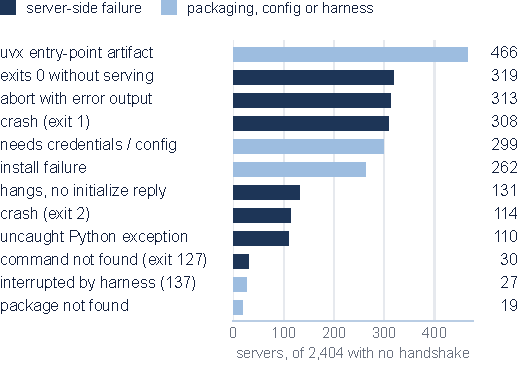
\includegraphics[width=\linewidth]{figures/failures.pdf}
  \caption{Why servers never reach a handshake. Configuration requirements and the
  entry-point artifact are separated from genuine startup failures.}
  \label{fig:failures}
\end{figure}

\begin{table}[t]
\centering
\caption{Startup-failure taxonomy: causes for servers that never reach a handshake.}
\label{tab:startup}
\begin{tabular}{lrr}
\toprule
Failure class & Count & \% of failures \\
\midrule
entrypoint-not-provided & 466 & 19.4 \\
exit-silent & 319 & 13.3 \\
crash-with-error-output & 313 & 13.0 \\
crash-exit-1 & 308 & 12.8 \\
needs-auth-or-config & 299 & 12.4 \\
install-error & 262 & 10.9 \\
hang-no-reply & 131 & 5.4 \\
crash-exit-2 & 114 & 4.7 \\
crash-python-exception & 110 & 4.6 \\
crash-exit-127 & 30 & 1.2 \\
crash-exit-137 & 27 & 1.1 \\
install-not-found & 19 & 0.8 \\
unclassified & 2 & 0.1 \\
crash-exit-255 & 1 & 0.0 \\
crash-exit-3 & 1 & 0.0 \\
crash-exit-4 & 1 & 0.0 \\
crash-exit-254 & 1 & 0.0 \\
\midrule
Total non-handshaking & 2404 & 100.0 \\
\bottomrule
\end{tabular}
\end{table}

\subsection{RQ2--RQ3: Conformance and robustness}
Table~\ref{tab:verdicts} reports the verdict distribution for each check over the
\Nresponders{} responding servers, with 95\% Wilson confidence intervals. Lifecycle
and tool-listing conformance are high, and the discriminating checks are error handling,
argument type enforcement, and malformed-input survival. \NoTypecheckRate{} of
responders failed to reject a wrong-typed required argument, which
Section~\ref{sec:consequences} decomposes into the servers that reported the problem
anyway and the smaller class that did not. \MalformedDiesRate{} failed to recover from a
malformed frame. We classify that as a robustness and conformance failure. The
security reading does not survive the transport: under stdio the client is the parent
process and the sole writer to the server's standard input, and a party able to
deliver a malformed frame can already terminate the subprocess. JSON-RPC 2.0, on which MCP is built,
nonetheless defines a parse-error response for this case and requires a reply to
every subsequent request~\cite{jsonrpc}, and these servers give neither. One
maintainer who reproduced the finding made this argument, and the classification here
follows it (Section~\ref{sec:threats}).

\begin{table}[t]
\centering
\caption{Verdict distribution per check over responding servers, with 95\% Wilson CIs on the pass (or documented) rate.}
\label{tab:verdicts}
\begin{tabular}{lrrrr}
\toprule
Check & Pass & Fail & Other & Pass rate (95\% CI) \\
\midrule
server-initialize & 217 & 0 & 0 & 100.0 (98.3--100.0) \\
ping & 216 & 1 & 0 & 99.5 (97.4--99.9) \\
tools-list & 215 & 2 & 0 & 99.1 (96.7--99.7) \\
tools-schema-valid & 214 & 1 & 0 & 98.6 (96.0--99.5) \\
tools-call-unknown & 7 & 12 & 198 & 3.2 (1.6--6.5) \\
tools-call-invalid-args & 197 & 15 & 5 & 90.8 (86.2--94.0) \\
malformed-json & 215 & 2 & 0 & 99.1 (96.7--99.7) \\
stdout-purity & 217 & 0 & 0 & 100.0 (98.3--100.0) \\
\bottomrule
\end{tabular}
\end{table}

\subsection{RQ3 refined: what a failure to reject actually returns}
\label{sec:consequences}
The \texttt{tools-call-invalid-args} verdict records whether a server rejects an
argument that violates its own declared schema. As a protocol judgment that
is correct, but it cannot tell a client what it received, because two different
behaviors produce the same verdict. A server may validate the input and
report the problem in the result \emph{text} without setting \texttt{isError}, which
is non-conformant but leaves the information available. Or it may execute the tool
and return ordinary-looking output, which does not. We separate the two by
classifying the recorded response of every server in this category
(Figure~\ref{fig:consequences}, Table~\ref{tab:consequences}).

\begin{figure}[t]
  \centering
  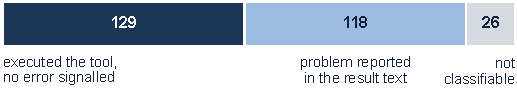
\includegraphics[width=\linewidth]{figures/consequences.pdf}
  \caption{The coarse verdict splits in half. Only the left segment is undetectable
  by the client: the tool ran on input its schema rejects and returned a well-formed
  result carrying no error indication.}
  \label{fig:consequences}
\end{figure}

Of \NAcceptInvalid{} such servers, \NInBandError{} (\InBandShare{}) reported the
problem in the result text, so the server noticed and a client willing to parse prose
could too. \NSilentExec{} (\SilentExecShare{}) executed the tool and returned a
result with no indication that anything was wrong. For \NUnclassifiable{} the
response could not be classified from the transcript. The hazard class is therefore \SilentExecRate{} of responding servers, smaller than the \NoTypecheckRate{} of the raw verdict, and it is the figure we report. We
count a server as reporting the problem whenever its output contains any error-like
token, so \NSilentExec{} is a lower bound.

This is not a matter of interpretation. The
specification's security requirements state that servers \textbf{MUST} validate all
tool inputs~\cite{mcpspec}. A server that executes a tool on an argument contradicting
its own published schema has not validated that input, so these \NSilentExec{} servers
fail an explicit RFC-2119 requirement, as do the servers that write non-protocol output to stdout, which the stdio transport forbids with a \textsf{MUST NOT}.

Here SDK attribution narrows the cause further than it does for the
error-reporting divergence. \SilentExecTS{} of the \NSilentExec{} are built on
the official TypeScript SDK and \SilentExecPy{} on either Python SDK, against
responding populations of \SDKPopTS{} and \SDKPopPy{} respectively. A behavior absent from one
language ecosystem and concentrated in another points to the library, so we tested the SDKs directly (Section~\ref{sec:sdk-probe}). On
\texttt{@modelcontextprotocol/sdk} 1.30.0, the current release at the time of writing,
a server built with the low-level \texttt{Server} API publishes an
\texttt{inputSchema} in \texttt{tools/list} and the SDK then does not check
\texttt{tools/call} arguments against it: a tool declaring a string property, called
with an integer, runs and returns a well-formed result. The same tool built with the
high-level \texttt{McpServer} API, whose schemas carry type information the SDK
already validates, rejects the identical call with an \texttt{isError} result. We did
not test the Python SDKs under the same conditions, so we report their absence from this population as an observation only. Within
the TypeScript SDK the gap is that one supported construction path publishes a
contract the library never enforces, so the servers on it have not declined a check
the SDK offered them. Of the \SilentExecTS{} TypeScript-SDK servers,
\SilentExecTSCaret{} declare a caret range and none declares an exact version.
Because each server was installed fresh, those ranges resolve to the newest 1.x, so this is current behavior, and a fix on the 1.x line
would reach almost all of them at their next install.

The unknown-tool divergence has a merged fix that deployed servers do not show. The
SDK's tracker records tool resolution as corrected in March 2026, four months before
our crawl, by a change that moves the tool-not-found check outside the handler's
\texttt{try} block so it propagates as a protocol error~\cite{sdkpr1389,sdkissue1510}.
We rebuilt the minimal high-level server on releases 1.28.0, 1.29.0 and 1.30.1 and
sent the same unknown-tool call. All three answer with an \texttt{isError} result
whose text reads \texttt{MCP error -32602: Tool \ldots{} not found}. The protocol
error is raised and then delivered inside a successful response, where a client
branching on JSON-RPC errors cannot see it. This explains a puzzle in our own data:
the census ran after the fix shipped, and the rate did not move.

The low-level path loses the tool name as well, which we had not tested. That API
takes one handler for every \texttt{tools/call} request, and the handler receives the
requested name without the library checking it against the declared tool list. Our
probe asked a low-level server for a tool it does not have and received that server's
ordinary answer, reporting a clean scan of code it was never given. Nothing in the
response marks the tool as missing.

In the recorded responses, a code-scanning tool asked to
scan the integer \texttt{12345} answered \texttt{CLEAN}, a prompt-scoring tool returned
a complete rubric including per-dimension sub-scores for the same integer, and a project
registry confirmed that a project named \texttt{12345} had been registered. All three are well-formed successful results. None relates to the question asked,
and at the protocol level none can be told apart from a correct answer: there is no
error code and no \texttt{isError} flag. Each server published a schema that would
have caught the call and then left it unenforced.

\begin{table}[t]
\centering
\caption{Servers that executed a tool on an argument their own declared schema
rejects, and returned ordinary-looking output. Inputs are the harness's type-poisoned
values; outputs are verbatim, truncated. None carries an error indication a client
could act on.}
\label{tab:consequences}
\small
\begin{tabular}{p{0.30\linewidth}p{0.20\linewidth}p{0.42\linewidth}}
\toprule
Tool & Argument sent & Result returned to the client \\
\midrule
\texttt{scan\_code\_imports} & \texttt{code: 12345} &
``CLEAN --- No npm package imports found in the provided code'' \\
\addlinespace
\texttt{register\_project} & \texttt{name: 12345} &
``Project 12345 registered successfully. Framework: generic'' \\
\addlinespace
\texttt{score\_prompt} & \texttt{prompt: 12345} &
a complete scoring rubric: \texttt{score: 8}, \texttt{grade: "F"}, with per-dimension
sub-scores \\
\addlinespace
\texttt{upcoming\_deadlines} & \texttt{within\_days: "not-a-number"} &
a dated regulatory snapshot with a populated result envelope \\
\addlinespace
\texttt{search} & \texttt{query: 12345} &
\texttt{\{"results":[]\}} \\
\bottomrule
\end{tabular}
\end{table}


\subsection{RQ4: Where practice and specification disagree, and which one moved}
\ErrAsResultRate{} of responding servers reported a call to a non-existent tool as an
\texttt{isError} tool-execution result instead of a JSON-RPC protocol error. The
specification's error-handling section lists ``unknown tool'' under \emph{Protocol
Errors} and illustrates it with a \texttt{-32602} example~\cite{mcpspec}. It attaches
no RFC-2119 keyword. We record which mechanism each server uses and score neither
as a violation (Section~\ref{sec:threats}).

The specification has been moving toward what servers do. SEP-1303, now
accepted and reflected in the specification, reclassified input validation errors from
protocol errors to tool execution errors on the grounds that a model can only
self-correct from an error it can see~\cite{sep1303}. SEP-2145, open at the time of
writing, proposes the same move for tool resolution failures, covering unknown and
disabled tools, and gives as its rationale that it ``aligns specification with existing
Python and TypeScript SDK behavior''~\cite{sep2145}. Our census measures how much of
the deployed ecosystem that alignment already describes: \ErrAsResultRate{} of
responding servers. (Aggregate figures from this census were posted to the
proposal's discussion thread while it was open.) The other \NotErrAsResultPct{} are
not one population: \UnknownProtoErrCount{} servers emit a protocol error coded
\texttt{-32602} or \texttt{-32601}, \UnknownWrongCodeCount{} use some other code, and
\UnknownProseCount{} return a plain success that states the failure only in its text,
a mechanism neither proposal describes.

To explain the uniformity, we attribute each server to its SDK from its resolved
dependency graph (Figure~\ref{fig:sdk}, Table~\ref{tab:sdk}). We take the exact
package version the probe launched and resolve its runtime dependencies through
deps.dev, so a server that reaches an SDK through a third-party wrapper is credited
to that SDK and not to the residual. \SDKDirect{} servers depend on an SDK directly
and \SDKIndirect{} reach one only through a wrapper. For \SDKUnattributed{} we have
no graph: the package or the probed version has since been withdrawn from its
registry. The behavior tracks the SDK: the
official TypeScript and Python SDKs and the FastMCP framework all default to it. A
small number of TypeScript-SDK servers emit the protocol error, so the alternative is
reachable within the SDK and simply is not the default. The official reference servers
behave the same way.

Our attribution recognizes a fixed list of known SDK package names, so the residual
\textsf{no-known-SDK} category holds servers with none of those names anywhere in
their runtime graph. Such a server may still have vendored an SDK at build time.
Resolving the graph transitively moves servers that inherit an SDK through a wrapper
into that SDK's family. That leaves the residual as the sharpest contrast in the
table: \SDKNoSDKRate{} of its \SDKNoSDK{} servers answer an unknown tool with an
\texttt{isError} result, against about nine in ten in every official-SDK family.
A few SDK defaults, used directly or through wrappers, account for this behavior
across the ecosystem. Where they are absent, so is the behavior.

\begin{figure}[t]
  \centering
  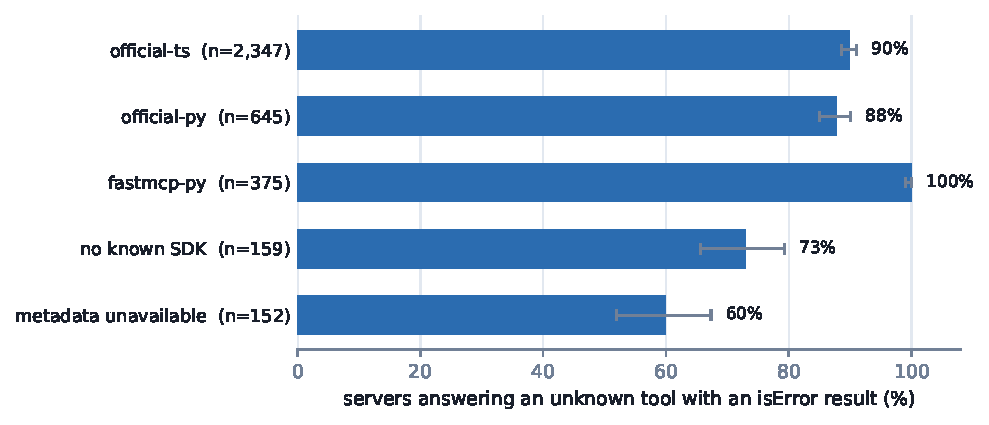
\includegraphics[width=\linewidth]{figures/sdk.pdf}
  \caption{Unknown-tool responses by SDK family. In every family, most servers answer with an \texttt{isError} result. Bars show 95\% Wilson intervals;
  families with fewer than 25 servers appear in Table~\ref{tab:sdk} only.}
  \label{fig:sdk}
\end{figure}

\begin{table}[t]
\centering
\caption{SDK family vs.\ unknown-tool response. Which mechanism a server uses tracks the SDK it was built on, not the author.}
\label{tab:sdk}
\begin{tabular}{lrrr}
\toprule
SDK family & error-as-result & protocol error & other \\
\midrule
official-ts & 2211 & 65 & 173 \\
official-py & 567 & 0 & 82 \\
fastmcp-py & 378 & 0 & 0 \\
no-known-SDK & 86 & 63 & 33 \\
metadata-unavailable & 16 & 2 & 0 \\
fastmcp-ts & 0 & 8 & 0 \\
xmcp-ts & 0 & 1 & 0 \\
\bottomrule
\end{tabular}
\end{table}

\subsection{RQ5: Correlates}
\label{sec:rq5}
We test whether runnability and conformance correlate with the package registry
(Figure~\ref{fig:byregistry}). Runnability differs: npm servers complete a
handshake far more often than PyPI servers (\NpmRate{} of \NpmN{} against
\PypiRateRaw{} of \PypiN{}, a difference of \GapRunnableCl{}). Conformance does not:
the same publisher-cluster bootstrap puts the error-as-result difference at
\GapErrAsResultCl{}, an interval spanning zero. We apply one method to both
comparisons so that neither rests on a stronger footing. The pattern follows from RQ4: because the
divergence is inherited from the SDKs, and both language ecosystems' SDKs share the
same default, the registry a server ships on changes whether it \emph{starts} but not
whether it \emph{conforms}.

Part of this gap came from our own launcher, and we corrected for it. We launch PyPI servers as \texttt{uvx <package>}, which resolves only
if the package's console script is named after the package; npm's \texttt{npx}
resolves the entry point from \texttt{package.json} and has no such requirement.
\NEntrypointBlocked{} PyPI servers (\EntrypointBlockedPct{} of the PyPI population)
installed successfully but were never launched for this reason alone. Our classifier
identifies \NEntrypointSeen{} such rows in the census; the completed re-probe covers
\NEntrypointBlocked{} of them, and \NEntrypointUnreprobed{} were missed. We
re-probed those servers with the entry point resolved from the installed package
metadata. \EntrypointRecovered{} (\EntrypointRecoveryRate{}) then completed a
handshake; the rest failed for reasons unrelated to naming (Python exceptions, hangs,
undeclared configuration). Correcting for this raises PyPI runnability from
\PypiRateRaw{} to \PypiRateCorr{} and the overall census figure to
\HandshakeRateCorr{}, which we report as the headline throughout. The npm--PyPI gap
narrows from \GapRaw{} to \GapCorr{} percentage points but stays large.

The entry-point problem is itself an ecosystem finding. Registry metadata does not
record a server's entry point, so a client following the registry alone cannot launch
a fifth of published PyPI servers, and once the entry point is resolved, nine in ten
of those servers still fail to start. A listing in the registry says
nothing about either.

\begin{figure}[t]
  \centering
  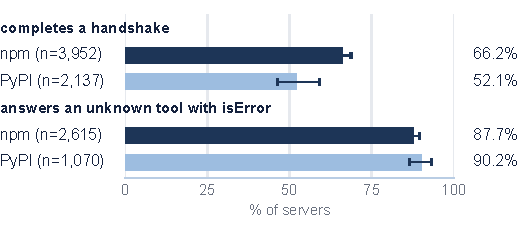
\includegraphics[width=\linewidth]{figures/by_registry.pdf}
  \caption{Handshake yield (PyPI after the entry-point correction) and the
  error-as-result rate for unknown tools, by package registry, with 95\% intervals
  from a publisher-cluster bootstrap.}
  \label{fig:byregistry}
\end{figure}
